\documentclass[10pt, a4paper]{article}
\usepackage[utf8]{inputenc}
\usepackage{geometry}
\geometry{margin=1in}
\usepackage{booktabs}
\usepackage[colorlinks=true, allcolors=blue]{hyperref}
\usepackage{setspace}
\usepackage{graphicx}
\usepackage{tabularx}
\usepackage{enumitem}
\usepackage[backend=biber]{biblatex}
\addbibresource{references.bib}
\setlength\bibitemsep{1pt}

\title{\textbf{Technical Report: Stress Prediction}}
\author{
    \textbf{Name:} Jack Hickey \\
    \textbf{Student ID:} 26257770 \\
    \textbf{Class:} 1MOA2 - CT5170\\
}
\date{}

\begin{document}

\maketitle
\onehalfspacing

\section{Understanding the Dataset}
The Stress-Predict Dataset is comprised of continuous physiological recordings captured from 34 participants using the Empatica E4. The primary objective of this task is to design, implement, and critically evaluate two machine learning hypotheses capable of inferring if an individual is stressed based on their respiration and heart rate levels.

The target label is binary where Label 0 indicates non-stressed and Label 1 indicates the participant is stressed. As we are dealing with categorical classes this excludes the need for regression, which aims to predict a value based on continuous data. Unsupervised learning would be suitable if the data were unlabeled. The purpose of this data is to predict a binary label based on mapping the heart and respiration rate to a label, making this an ideal candidate for supervised binary classification. 

\section{Data Exploration}
The dataset comprises 112,516 physiological recordings across 34 distinct participants. Inspection of feature integrity reveals that \texttt{respr}, \texttt{Time(sec)}, and \texttt{Label} contain complete records, while \texttt{HR} contains 44 missing values that require imputation or filtering during pre-processing.

Analysis of the target variable reveals moderate class imbalance with $\sim$67.28\% classed as 0 and $\sim$32.72\% classed as 1. The majority class accounts for roughly two-thirds of the observations, a trivial hypothesis defaulting to class 0 would achieve $\sim$67.3\% baseline accuracy. This means accuracy is insufficient on its own and model evaluation must incorporate Precision, Recall, and F1-score to measure the performance of the algorithm on the minority class \parencite{he2009learning}. Something worth considering is that physiological data can vary greatly across individuals and we lack information such as age, sex, weight, and other general health metrics that may play a role in what constitutes stressed in any individual. For example, participant 8 has a resting heart rate of $\sim$93 and participant 6 has a stressed heart rate of $\sim$75. This variance may prove difficult for a classification model.

% \begin{table}[h]
% \centering
% \begin{tabular}{@{}lcccc@{}}
% \toprule
% \textbf{Metric} & \textbf{Participant} & \textbf{Heart Rate (HR) [BPM]} & \textbf{Respiration Rate} & \textbf{Label} \\ \midrule
% Count & 112,516 & 112,472 & 112,516 & 112,516 \\
% Min & 2 & 49 & 5.2 & 0 \\
% Max & 35 & 146.78 & 18.16 & 1 \\ \bottomrule
% \end{tabular}
% \caption{Descriptive statistics of the dataset features.}
% \end{table}

\section{Choosing an ML Package}
Several open-source packages support classification workflows across different areas:
\begin{itemize}
    \item \textbf{Scikit-Learn (Python):} The standard open-source library for classical, tabular machine learning, offering tools for pre-processing, classification, regression, clustering, and model validation.
    \item \textbf{TensorFlow:} Deep learning framework designed for high-dimensional, unstructured data.
    \item \textbf{WEKA:} A popular Java based library with a GUI offering implementations of classical learners like C4.5 decision trees.
\end{itemize}

Scikit-Learn is selected as the primary library for this assignment due to several key features:
\begin{enumerate}
    \item \textbf{Unified and Consistent API:} The API adheres to a standard interface that is easy to use and consistent across algorithms simplifying comparisons between different classifiers.
    \item \textbf{CRISP-DM Workflow:} It provides native utilities for all stages of the CRISP-DM lifecycle, including participant splitting, data transformation and scaling, and algorithmic modeling.
    \item \textbf{Comprehensive Metric Suite:} Built-in functions like \texttt{f1\_score} allow direct handling and evaluation of imbalanced classification problems without external dependencies.
\end{enumerate}

\section{Data Pre-processing}
Examining the dataset reveals 44 missing values within the \texttt{HR} column. While mean or median imputation is a common strategy, injecting static values into continuous physiological time-series data can create artificial flatlines \parencite{hayat2021missing, little2019statistical}.
Given that 44 rows is a negligible fraction of the total entries, dropping these rows entirely is a safe approach to maintain data integrity.

To prevent data leakage caused by correlating sequential time-series entries from the same individual, the train/test split was performed at the participant level rather than by random row shuffling \parencite{saeb2017need}. Applying an 80/20 subject split allocates 27 participants to the training set and 7 participants to the test set. After dropping the 44 rows with no Heart Rate value  that leaves 90,034 rows in the training samples and 22,438 in the testing samples.

 The \texttt{Participant} column is removed from the feature set as retaining it could allow the algorithm to associate a specific participant ID directly with a stress state, leading to severe overfitting. The \texttt{Time(sec)} column is also removed as it serves merely as an index and provides no independent predictive value for identifying stress states.

To prepare the remaining physiological features (\texttt{HR} and \texttt{respr}) for k-NN, feature scaling is required. Distance metrics such as Euclidean or Manhattan evaluate all dimensions equally. Therefore, without scaling, Heart Rate would mathematically dominate Respiration during distance calculations. To resolve this, I applied Z-Normalisation and Range-Normalisation independently for comparative purposes both of which put the features on comparable scale. 

\section{Algorithm Selection and Application}
To evaluate predictive performance across distinct machine learning paradigms, two supervised classification algorithms were selected and applied to the pre-processed physiological dataset: Decision Trees and k-Nearest Neighbour (k-NN) \parencite{hastie2009elements}.

\begin{enumerate}
    \item \textbf{Decision Trees (Eager Learning):} Decision Trees construct an inverted tree structure by continuously partitioning the feature space based on feature splits until a leaf node with no further splits is formed. During training, the algorithm evaluates potential splits using criteria such as Gini Impurity or Shannon Entropy to maximise information gain at each node \parencite{ullah2025topic2}. % To prevent overfitting and promote generalisation on unseen subject data, hyperparameter tuning can be conducted across tree depth constraints, minimum sample requirements for leaf nodes, and class weighting to address dataset class imbalance.
    \item \textbf{k-Nearest Neighbours (k-NN, Lazy Learning):} Unlike eager learners k-NN defers computation until inference time by storing the normalised training vectors. When classifying an unlabelled physiological observation, the algorithm identifies the $k$ most similar instances using a distance metric such as Euclidean or Manhattan distance and assigns the class label via majority voting \parencite{ullah2025topic3}. %Model optimisation can involve evaluating varying neighborhood sizes across Minkowski distance metrics, testing both uniform weighting and distance-inverse weighting rules to prioritise closely adjacent training points.
\end{enumerate}

\section{Model Evaluation}
Models were evaluated across five metrics:
\begin{itemize}
    \item \textbf{Accuracy:} The total number of correct predictions divided by the total predictions.
    \item \textbf{Precision Score:} When the model predicted stressed, how many times it was right.
    \item \textbf{Recall:} How many of the actual stress events in the dataset the model successfully caught.
    \item \textbf{F1 Score:} The harmonic mean of precision and recall, giving a more balanced answer when dealing with imbalanced datasets.
    \item \textbf{Time:} A measure of the computational cost of an algorithm.
\end{itemize}

Initial results without any hyperparameter tuning on both k-NN and Decision Trees resulted in scores hovering around our baseline score, and the F1 Score reveals that the algorithms simply went with the majority class.

\textbf{k-Nearest Neighbour:}\\
Analysing differences across Z-Normalisation and Range Based Normalisation showed negligible differences across all $k$ and $p$ values. The dataset relies on a two dimensional feature space without extreme, isolated outliers that would drastically skew a Range Based transformation, so both techniques provided nearly identical results. This meant the nearest neighbors for any given query point under each were nearly the same. 

As $k$ increases from 1 to 100, Accuracy steadily climbs from $\sim$55\% to $\sim$60\%. Concurrently, F1-score drops from 0.3550 down to 0.2795, and Recall falls from $\sim$36\% to $\sim$22\%. Because the dataset is roughly two-thirds Class 0, expanding the neighborhood radius makes it increasingly likely that the local majority will outvote the minority class. Distance metrics across Manhattan, Euclidean and Minkowski ($p=4$) had minimal impact. The curse of dimensionality is absent in a 2D feature space, causing the different distance norms to maintain similar neighborhood boundaries. Testing of distance weighting rules also didn't help and this is likely because the variability in participants stress and not stressed states was too much meaning 1 person's stressed state was another's non-stressed baseline.

\textbf{Decision Trees:}\\
Decision trees using Gini Impurity and Shannon Entropy were evaluated against each other. The result was both constructed nearly identical tree structures, which meant no performance variance. In a two dimensional feature space they produce nearly identical splits in data.

Testing of pruning through tree depth alone did not give positive results. A tree depth of 1 confirmed our hypothesis that defaulting to the majority class gives a baseline accuracy of $\sim$67\%. While this was the most accurate model, its F1 score was 0, rendering it useless for actual stress prediction. To prevent the model from defaulting to Class 0, \texttt{class\_weight='balanced'} was combined with tree depth and minimum leaf size constraints. This combination resulted in the best model with an equal Accuracy and F1 score of $\sim$50\% (achieved using Gini, \texttt{max\_depth}=6, \texttt{min\_samples\_leaf}=5). Unfortunately, this performance remains well below the baseline standard.

\section{Comparative Analysis}
\begin{figure}[h]
    \centering
    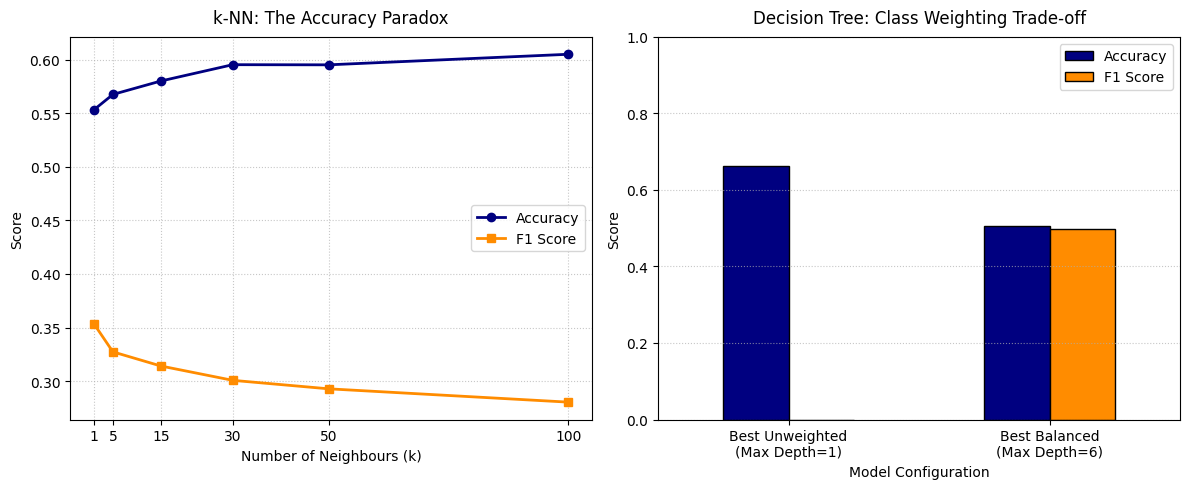
\includegraphics[width=0.82\textwidth]{model_evaluation.png}
    \caption{Left: The Accuracy Paradox in k-NN. Right: Decision Tree comparison of the most accurate left with the best balance of accuracy and F1 score right.}
    \label{fig:model_evaluation}
\end{figure}

Both the k-Nearest Neighbours and Decision Tree algorithms ultimately hit a $\sim$50-60\% accuracy ceiling despite extensive hyperparameter tuning and distance/class weighting. While the unconstrained models achieved higher absolute accuracy ($\sim$66\%), this was a reflection of the Accuracy Paradox, where the algorithms minimised error by defaulting to the majority non-stressed class, effectively failing to detect the minority stress events entirely.

Implementing \texttt{class\_weight='balanced'}, \texttt{max\_depth}=6, and \texttt{min\_samples\_leaf}=5 altered the decision boundary of the Decision Tree. This forced the tree to aggressively predict the stress class, successfully driving up Recall and the F1-Score, but at the strict cost of overall Accuracy.

Ultimately, both algorithms succumbed to the inherent limitations of the feature space. Instantaneous \texttt{HR} and \texttt{respr} readings lack the necessary context to definitively isolate a stress response. Furthermore, variance in human physiology means that a generalised model often fails to account for individual baseline differences. Future attempts would address these limitations through two distinct shifts. First, integrating time through rolling variances would capture the physiological development of stress over time prior to algorithmic classification \parencite{tds_timeseries_rolling}. Second, transitioning from generalised modeling to participant-specific classifiers would allow the algorithm to infer stress based entirely on an individual's unique physiological baseline.
% Both the k-Nearest Neighbours and Decision Tree algorithms ultimately hit a $\sim$50-60\% accuracy ceiling despite extensive hyperparameter tuning and distance/class weighting. While the unconstrained models achieved higher absolute accuracy ($\sim$66\%), this was a reflection of the Accuracy Paradox where the algorithms minimised error by defaulting to the majority non-stressed class, effectively failing to detect the minority stress events entirely.

% Implementing \texttt{class\_weight='balanced'}, \texttt{max\_depth}=6, \texttt{min\_samples\_leaf}=5) together altered the the prediction of the Decision Tree. This forced the tree to predict the stress class more often, successfully driving up Recall and the F1-Score, but at the cost of overall Accuracy.

% Both algorithms succumbed to majority bias. It may well be a result that \texttt{HR} and \texttt{respr} alone are not sufficient enough to predict stress levels or it may be that the variance in human physiology means individuals metrics do not map to others. If I was to approach this in the future I may consider time through techniques such as rolling variances to capture the development of stress over time prior to algorithmic classification \parencite{tds_timeseries_rolling}. This fell out of the scope of this as it is a technique I learned about late in the analysis. Another consideration I had late in the analysis was instead of trying to map a participants physiological data to another participants for making predictions I could split the data of each individual participant and try to infer if that participant is stressed based on their individual physiological data.


\begingroup
\footnotesize
\printbibliography
\endgroup

\end{document}
